\cleardoublepage

\addcontentsline{toc}{chapter}{\numberline{}4eme chapiter}
\addtocontents{lof}{\textbf{Chapter A4}}

\setcounter{chapter}{4}
\setcounter{section}{0}
\setcounter{figure}{0}
%\setcounter{algorithm}{0}

\begin{center}
	\Huge\textbf{4eme chapter}
\end{center}

\section{Introduction}
Dans les chapitres précédents, nous avons introduit différentes techniques utilisées pour la résolution des problèmes d’optimisation combinatoire, notamment les méthodes adoptées pour la résolution du problème de l’arbre dominant DTP, dont une grande majorité a servi de source d’inspiration pour l’élaboration des approches que nous avons proposé et qui seront détaillées le long de ce chapitre.  Nous allons dans un premier présenter les structures de données utilisées pour représenter les données du problème ainsi que la solution.

\section{Représentation du graphe modélisant le problème}
Un WSN est un graphe pondéré non orienté $G=(V,E,w)$, où $V$ est l’ensemble des nœuds du réseau, E l’ensemble des arêtes et w un poids non négatif attribué pour chaque arête $e=(u,v)$. 

Nous utilisons pour représenter le WSN deux vecteurs, un vecteur de taille $|V|$ contenant des entiers représentant chaque nœud et l’autre est de taille $|V-1|$ il contient une structure d’arc (nœud 1, nœud 2 et le poids entre les deux nœuds. Nous allons dans ce qui suit présenter le codage de la solution ainsi que la méthode d'extraction du DT à partir de cette solution.


\section{présentation d’une solution:}
Nous proposons de représenter une solution en utilisant le codage binaire qui est considéré dans la littérature comme un bon moyen pour manipuler les différents gène (position(bit) dans une solution) d’une solution pour une population donnée. Si le gène est égale à '1', cela veut dire que le nœud correspondant est actif, s'il vaut '0', il est inactif.


\section{Méthode d'extraction d'un arbre dominant à partir du vecteur solution:}
Au départ nous avons deux vecteurs $(Vect, DN)$, où, $Vect$ contient tous les nœuds de notre graphe, $DN$ est un vecteur binaire de taille $|V|$ initialement null et contiendra par la suite l’ensemble des nœuds dominant .

L’ajout des nœuds à $DN$ se fait via un processus itératif. A chaque fois un nœud est choisi d’une façon aléatoire,  et est ajouté à $DN$. Ce processus poursuit son fonctionnement tant que les nœuds appartenant à $DN$ ne couvre pas tous le graphe ou ils ne sont pas  connectés. On dit que $DN$ couvre le graphe si et seulement si tous les nœuds de notre graphe sont soit dans $DN$ soit adjacent à un autre nœud qui est dans $DN$.

Pour pouvoir construire un DT, il faut d’abord vérifier  que les nœuds actifs dans $DN$  sont connectés entre eux. Dans le meilleur des cas, les nœuds actifs dans $DN$ sont connectés ; Dans le cas contraire nous devons les rendre connecté en utilisant une méthode de connection décrite si après.

\section{La méthode de connection:}
Soit un vecteur DNC initialement vide qui va contenir par la suite ensemble de nœuds connecté. En premier lieu, nous retirons un nœud aléatoirement de DN et nous l’insérons dans DNC. Puis, d’une façon itérative, nous retirons tous les nœuds de DN qui ont au moins un voisin dans DNC et nous l’insérons dans DNV. En second lieu nous, devons insérer tous les nœuds actifs dans DN dans DNC en utilisant une autre fonction. Cette fonction consiste au départ, à choisir un nœud v aléatoirement dans V qui n’est pas dans DNC. Si v a au moins deux voisins un dans DN et l’autre dans DNC, alors nous retirons son voisins dans DN et nous l’insérons  avec v dans DNC. Si aucun nœud n’est trouvé nous procédons à une sélection par pair de nœuds où chaque nœud entre eux a soit un voisin dans DN ou dans DNC et nous refaisions le même processus de recherche daans le cas d’un seul nœud à selectionner. Nous ré-exécutons ce prceossus jusqu'à DN devient null.

Une fois que l’ensemble DN soit null, nous appliquant la méthode d’élagage et MST décrit dans le chapitre 3. Nous aurons au final, un arbre dominant DT, représenté sous forme d’un vecteur de type arc (chaque élément de ce vecteur est composé d’un noeud1, noeud2, et le poids entre ces deux nœuds).


\section{Approche proposée:}
Dans ce mémoire nous avons proposé plusieurs approches pour résoudre le DTP. Nous avons proposé de le résoudre dans un premier temps en utilisant des méta-heuristiques, et en utilisant la coopération de ces méta-heuristiques dans un second temps. Nous allons structurer ce qui suit en deux parties. Dans la première partie, nous présentons chacune des méta-heuristiques utilisées, dans la seconde partie, nous présentons l'approche coopérative.


\subsection{description des méta-heuristiques utilisées}
La méthode de résolution du problème de l’arbre dominant que nous avons proposée consiste à intégrer un processus de recherche locale  à la méta-heuristiques. Nous allons dans ce qui suit décrire les approches proposées. 

\subsubsection{Ant colony optimisation}
Nous utilisons dans cette première solution, l'algorithme des colonies de Fourmies pour résoudre le DTP. Nous allons décrire dans ce qui suit l'adaptation des operateurs de  cette métaheuristique au problème étudié. 

\begin{enumerate}[label=\alph*)]
	\item \textbf{Recherche locale:}\\
	Dans la recherche locale que nous proposons, supposons que nous avons une solution. Nous parcourons le vecteur de la solution et on inverse la valeur des élément (si la valeur d’un élément est égale à 1, elle devient 0 ou inversement) . A chaque fois que nous inversons  la valeur  de chaque élément nous faisons une évaluation de la fonction objectif. A tous coups où la solution est améliorée, cette dernière est sauvegardé et la recherche d’une meilleure solution se fera à partir de cette solution.
	
La recherche se terminera lorsque touts  les nœuds dominants aurons été parcourus.
il est à noter que la méthode de recherche locale citée ci dessus est utilisée dans toutes les solutions proposées.
	
	\item \textbf{Les méthodes de sélection:}\\
	Nous proposons d'utiliser deux méthodes de sélection d’individus. Ces deux méthodes ont été retenues après une série d'expérimentations faisant apparaître les deux méthodes donnant les meilleurs résultats.

	\begin{itemize}
		\item \textbf{Méthode de sélection par Intensification: }\\
		Son principe consiste à choisir le nœud ayant la plus grande probabilité pour améliorer la solution 
		
		\item \textbf{La sélection par tournoi}\\
		le principe de cette sélection consiste à choisir deux nœuds aléatoirement, puis de retenir celui ayant la meilleure probabilité 
	\end{itemize}


\end{enumerate}


\subsubsection{Fonctionnement de l’algorithme ACO :}
L’algorithme de colonie de fourmi est une approche métaheuristique basée sur une  population et inspirée du comportement des fourmis réelles. L’idée principale derrière cette méthode provient de l’observation de la capacité des fourmis pour trouver le plus court chemin entre une  source de nourriture et le nid.
Cette méta-heuristique est composée d’une phase d’initialisation et d’une phase itérative. La première phase consiste à initialiser une solution de départ qui sera décrite ci-dessous. Elle comprend également l’initialisation du vecteur des probabilités et de la table de phéromone.

Ensuite, pour chaque itération, chaque fourmi construit sa solution en choisissant aléatoirement une méthode de sélection (intensification - sélection par tournois). Après avoir construit une solution la recherche locale est lancée pour atteindre un résultat meilleure. La meilleure solution retournée par la fourmi courante va participer à la mise à jour du vecteur de probabilité( mise à jour en ligne ) en appliquant la formule (1). A la fin de chaque itération, la meilleure solution trouvée par la population de fourmis va elle aussi participer à la mise à jour du vecteur de probabilité  (mise à jour hors ligne) avec la formule suivante:

\begin{equation}
	\mathlarger{
		p_{ij}^k = \frac{
				[T_j]^\alpha \, [n_{ij}]^\beta
			}{
				\mathlarger{\sum}_{h \in S} \, \mathlarger{\sum}_{l \in N_h^k} \, [T_l]^\alpha \, [n_{hl}]^\beta
			}
	}
\end{equation}


où:\\
$T_j$ la concentration de phéromone du nœud $j$ \\
$n_{ij}$ est le terme heuristique qui vaut $1 / w_{ij}$, dont $w_{ij}$ est le poids de l’arc du nœud $i$ vers le nœud $j$.\\
$\alpha \, , \beta$ sont deux paramètres qui déterminent l'influence relative de la trace de phéromone et de l'information heuristique dans le processus de génération des solutions. \\
$N_h^k$ est l'ensemble de sommets non sélectionnés adjacents à un sommet $h \in S$. \\

Nous allons décrire dans ce qui suit, l'approche de construction de la solution initiale. Soit S l'ensemble des solutions (initialement vide). Tous les sommets de notre graphe sont étiquetés initialement comme non marqués. Un sommet v est sélectionné aléatoirement dans l'ensemble V puis  ajouté à S. Ce sommet est étiqueté comme marqué et tous les sommets adjacents à ce sommet deviennent marqués. Après cela, à chaque étape, la fourmi k construit une solution en sélectionnant un sommet non sélectionné v adjacent à un sommet déjà sélectionné $u \in S$. La sélection de ce sommet non sélectionné v est déterminée de manière probabiliste.


Après que tous les sommets du graphe soient étiquetés à marqué. Les fonction élagage et MST décrit dans le chapitre 3 sont appliquées.\\

Le pseudo-code de ACO est donné dans l’algorithme 1 suivant:

\begin{algorithm}[H]
\caption{ACO de DT }
\KwData{Un graphe général pondéré non orienté $G = (V, E, w) $}
\KwResult{Un DT  optimal de G }
\SetAlgoLined
\DontPrintSemicolon

Initialiser le vecteur de probabilité ainsi que la table de pheromone \;
Construction de la solution initiale \;

\While{le nombre d’itération non atteint }{
	\For{chaque fourmi}{
		Construction d’une solution \;
		Recherche locale() \;
		Mise à jour de la table de phéromone. Selon la meilleure solution trouvée par la fourmi \;
	}
	Mise à jour de la table de phéromone Selon la meilleur solution atteinte par les fourmis\;	
}
	
\end{algorithm}



\subsubsection{Algorithme génétique}
Nous allons décrire dans ce qui suit les opérateurs retenus dans l'approche utilisant les algorithmes génétiques. 


\begin{enumerate}[label=\alph*)]
	\item \textbf{Génération de la Population initiale:}\\
	La population initiale est construite avec un ensemble de solutions (individu) définies aléatoirement. La taille de chaque individu est le même nombre de nœuds dans un réseaux de capteurs sans fil.


	\item \textbf{Codage des éléments d’une population: }\\
	Le codage utilisé dans cette approche est celui décrit dans la section II.
	
	\item \textbf{La méthode de croisement utilisée:}\\
	Pour cet algorithme nous avons utilisé la méthode de croisement uniforme. Il opère à l’aide d’un masque construit aléatoirement, pour décider lequel des parents va transmettre  la valeur du gène à l’un ou l’autre des descendants. Si à la même position que le gène, la valeur du masque est égale à 1, le gène du parent 1 passe à celui de l’enfant 1 et le gène du parent 2 passe à l’enfant 2. Sinon, c’est l’inverse qui se produit (figure 4.1). Cette fonction renvoie l’enfant ayant la meilleur qualité (le poids minimal).\\
La figure 4.1  illustre se processus par un exemple.

\begin{figure}[H]
	\centering
	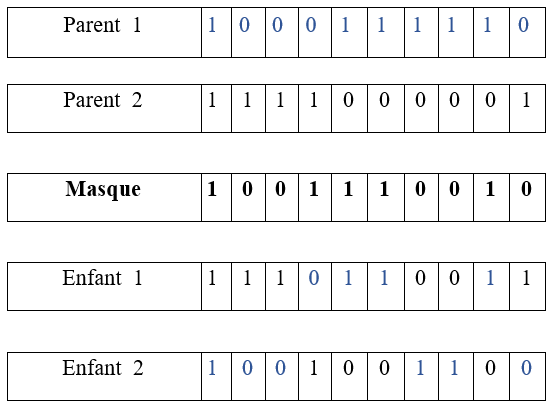
\includegraphics[width=12cm,height=6.5cm]{Chap4/1.png}
	\caption{Exemple de croisement uniforme}
	\label{fig:CSF}
\end{figure}
	

\end{enumerate}


